\item \textbf{{[}HCI/PRELIM/9597/2019/P1/Q3{]} }

The examinations department of a school needs to keep long-term records
of the overall examination achievements of its students.

Students at the school have two main choices. Firstly, they can take
a variety of subjects and achieve an Academic Diploma. A diploma gives
them the opportunity to go to university. Secondly they can achieve
a Skills Certificate where they focus on one particular area (such
as IT). This gives them the necessary skills to start a career in
their chosen area.

The examinations department decides to store the following data:
\begin{itemize}
\item \texttt{StudID} is used to uniquely identify a particular student
and is six digits. The first four digits represent the year that the
student started at the school and the last two digits are used to
make the \texttt{StudID} unique e.g. 201804.
\item \texttt{Name} is the name of the student and is at most 30 characters.
\item \texttt{StudType} is the type of student and can have the values \textquoteleft D\textquoteright{}
or \textquoteleft S\textquoteright .
\item \texttt{SkillArea} is text and gives the area that the student acquired
skills in. It can have one of three values: \textquoteleft IT\textquoteright ,
\textquoteleft Business\textquoteright{} or \textquoteleft Accountancy\textquoteright .
\item \texttt{NoOfSub} is the number of subjects studied by those taking
the Diploma. 
\item \texttt{Result} is a single character and is used to indicate the
overall grade awarded. For those students who took the Skills Certificate
the grades could be Distinction (D), Merit (M), Pass (P) or Fail (F).
For those who took the Diploma the grade could be one of the letters
A to F. Grade A to E are passes. Grade F is a fail.
\end{itemize}
The program design for a solution to this problem is to be implemented
with object-oriented programming with the following three classes:
\begin{center}
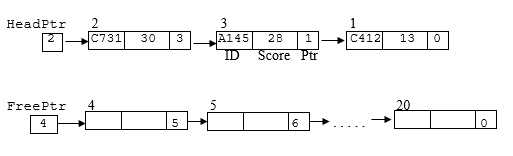
\includegraphics[width=0.5\paperwidth]{C:/Users/Admin/Desktop/Github/question_bank/LyX/static/img/9597-HCI-2019-P1-Q4-1}
\par\end{center}

\subsection*{Task 3.1 }

Write program code to define the classes \texttt{Student}, \texttt{Diploma}
and \texttt{SkillsCert}.

\subsection*{Evidence 8}

Program code for the three classes in Task 3.1. \hfill{}{[}6{]}

Assume that a file, \texttt{STUDENT.txt}, which contains details of
each student, has been created for you. The format of each student
record is as follows: 
\noindent \begin{center}
\texttt{<StudID>|<Name>|<StudType>|<SkillArea>|<NoOfSub>|<Result>}
\par\end{center}
\begin{itemize}
\item \texttt{SkillArea} would have the value \textquoteleft Diploma\textquoteright{}
if the student is taking a Diploma. 
\item \texttt{NoOfSub} would have the value 0 for those taking the Skills
Certificate.
\item \texttt{Result} is left blank initially. 
\end{itemize}

\subsection*{Task 3.2 }

Write a module, \texttt{ENTER\_RESULT}, which, when called, will ask
the user for a particular \texttt{StudID} whose result is to be entered.
Using the student ID that has been input, the corresponding student
record will be located in \texttt{STUDENT.txt}. The student data will
be displayed to the user. The user will be allowed to enter the result
for the student. The amended record will be stored back in \texttt{STUDENT.txt}. 

The student ID and result that have been input should be validated. 

If the \texttt{StudID} does not exist, the user will be given an appropriate
message.

\textbf{You are expected to make use of the classes you designed in
Task 3.1}.

Run the program \textbf{three} times. Use the following data input,
and produce a screenshot for each. 
\noindent \begin{center}
\begin{tabular}{cc}
StudID & Result\tabularnewline
\hline 
\texttt{201701} & \texttt{A}\tabularnewline
\texttt{201801} & \texttt{B}\tabularnewline
\texttt{201901} & \texttt{M}\tabularnewline
\end{tabular}
\par\end{center}

\subsection*{Evidence 9}

Program code for Task 3.2 \hfill{}{[}8{]}

\subsection*{Evidence 10 }

Three screenshots showing the test runs and final contents of \texttt{STUDENT.txt}
to show evidence that successful updates have been carried out. \hfill{}{[}2{]}

\subsection*{Task 3.3}

Implement code as specified below.

A report should be generated and displayed which will list the students
whose result has still not been entered into the \texttt{STUDENT.txt}
file. The report will list, for each different starting year: 
\begin{itemize}
\item \texttt{StudID} 
\item \texttt{Name} 
\item \texttt{StudType}
\item \texttt{SkillArea} or \texttt{NoOfSub} depending upon the value of
\texttt{StudType} 
\end{itemize}
In addition the number of each student type for each year will also
be output.

A sample output is shown below.
\noindent \begin{center}
\begin{tabular}{llll}
Year: 2017 &  &  & \tabularnewline
\hline 
\texttt{201715} & FLoo & D & 6\tabularnewline
\texttt{201708} & BLang & D & 5\tabularnewline
\texttt{201710} & LArms & S & IT\tabularnewline
Diplomas: & 2 &  & \tabularnewline
Skills: & 1 &  & \tabularnewline
\end{tabular}
\par\end{center}

\noindent \begin{center}
\begin{tabular}{llll}
Year: 2018 &  &  & \tabularnewline
\hline 
\texttt{201813} & FJean & D & 7\tabularnewline
\texttt{201817} & ABright & D & 7\tabularnewline
Diplomas: & 2 &  & \tabularnewline
Skills: & 0 &  & \tabularnewline
\end{tabular}
\par\end{center}

\noindent \begin{center}
\begin{tabular}{llll}
Year: 2019 &  &  & \tabularnewline
\hline 
\texttt{201905} & Alfie & S & Business\tabularnewline
\texttt{201903} & GKoh & D & 8\tabularnewline
Diplomas: & 1 &  & \tabularnewline
Skills: & 1 &  & \tabularnewline
\end{tabular}
\par\end{center}

\subsection*{Evidence 11 }

Program code for Task 3.3. \hfill{}{[}8{]}

\subsection*{Evidence 12 }

Screenshot of the output produced.\hfill{} {[}2{]}